\documentclass[8pt, twocolumn]{article}
\usepackage[margin=1in]{geometry}
\usepackage{lmodern}% http://ctan.org/pkg/lm
\usepackage{authblk} % adds affiliations

\usepackage[utf8x]{inputenc}
\usepackage{nameref}
\usepackage[switch]{lineno}
\usepackage{amsmath}
\usepackage{booktabs}
\usepackage[numbers,super]{natbib}
\usepackage{changepage}

% for pseudocode
\usepackage[]{algorithm2e}


% adjust caption style
\usepackage[aboveskip=1pt,labelfont=bf,
            labelsep=period,singlelinecheck=off]{caption}

% remove brackets from references
\makeatletter
\renewcommand{\@biblabel}[1]{\quad#1.}
\makeatother

\usepackage[colorinlistoftodos]{todonotes}

% headrule, footrule and page numbers
\usepackage{lastpage,fancyhdr,graphicx}
\usepackage{epstopdf}
\pagestyle{myheadings}
\pagestyle{fancy}
\fancyhf{}
\rfoot{\thepage/\pageref{LastPage}}
\renewcommand{\footrule}{\hrule height 2pt \vspace{2mm}}

% use \textcolor{color}{text} for colored text (e.g. highlight to-do areas)
\usepackage{color}

\definecolor{Gray}{gray}{.25}

\usepackage{graphicx}

% use if you want to put caption to the side of the figure
\usepackage{sidecap}

\usepackage{xcolor}
\usepackage[colorlinks = true,
            linkcolor = blue,
            urlcolor  = blue,
            citecolor = blue,
            anchorcolor = blue]{hyperref}

% ####################################################
% ####################################################
\usepackage[colorinlistoftodos]{todonotes}
% ####################################################
% ####################################################

% use for have text wrap around figures
\usepackage{wrapfig}
\usepackage[pscoord]{eso-pic}
\usepackage[fulladjust]{marginnote}
\reversemarginpar{}

\usepackage{gensymb}
\usepackage{siunitx}

% make a box for author summary
\usepackage[framemethod=TikZ]{mdframed}
%% define the style
\newcommand{\mybox}[2]{%
         \begin{center}%
            \begin{tikzpicture}%
                \node[rectangle, draw=#1, top color=#1!10, bottom color=#1!10,
                      rounded corners=5pt, inner xsep=5pt, inner ysep=6pt,
                      outer ysep=10pt]{
                        \begin{minipage}{1\textwidth}#2\end{minipage}};%
            \end{tikzpicture}%
         \end{center}%
}

% new commands
% q value
\newcommand{\qval}[1]{$q<10^{-#1}$}

% species names
\newcommand{\cel}{\emph{C.~elegans}}
\newcommand{\dicty}{\emph{D.~discoideum}}
\newcommand{\ecol}{\emph{E.~coli}}
\newcommand{\gf}{gain-of-function allele}
\newcommand{\lf}{loss-of-function allele}
\newcommand{\strong}{strong loss-of-function allele}
\newcommand{\weak}{weak loss-of-function allele}

% gene names
% \newcommand{\gene}[1]{\emph{#1}} # for MS word typesetting
\newcommand{\gene}[1]{\mbox{\emph{#1}}}
\newcommand{\genotype}[1]{\mbox{\emph{#1}}}
\newcommand{\protein}[1]{\mbox{\uppercase{#1}}}
\newcommand{\ras}{\gene{let-60} (\emph{ras})}
\newcommand{\rasp}{\protein{let-60}}
\newcommand{\dpy}[1]{\gene{mdt-12#1}}
\newcommand{\letgfn}{3,021}
\newcommand{\letlfn}{857}
\newcommand{\letgf}{\gene{let-60(gf)}}
\newcommand{\letlf}{\gene{let-60(lf)}}
\newcommand{\strongn}{2,863}
\newcommand{\weakn}{481}
\newcommand{\transn}{2,214}
\newcommand{\bx}{\dpy{(bx93)}}
\newcommand{\sy}{\dpy{(sy622)}}

% more space between rows
\newcommand{\ra}[1]{\renewcommand{\arraystretch}{#1}}

\title{A study of allelic series using transcriptomic phenotypes}

\author[1]{David Angeles-Albores}
\author[1,*]{Paul W. Sternberg}
\affil[1]{Division of Biology and Biological Engineering, Caltech,
Pasadena, CA, 91125, USA}
\affil[*]{Corresponding author. Contact: pws@caltech.edu}
\renewcommand\Affilfont{\itshape\small{}}

% document begins here
\begin{document}
% title

\twocolumn[
  \begin{@twocolumnfalse}
    \maketitle
    % \section*{Abstract}
    \textbf{Although transcriptomes have recently been used to perform epistasis
    analyses, they are not yet used to study intragenic function/structure
    relationships. We developed a theoretical framework to study allelic
    series using transcriptomic phenotypes. As a proof-of-concept, we apply our
    methods to an allelic series of \dpy{}, a highly pleiotropic Mediator subunit
    gene in \emph{Caenorhabditis~elegans}. Our methods identify functional units
    within \dpy{} that modulate Mediator activity upon various genetic modules.
    }
    \vspace{3mm}

  \end{@twocolumnfalse}
]


\linenumbers{}
\section*{Introduction}
Mutations of a gene can yield a series of alleles with different phenotypes that
reveal multiple functions encoded by that gene, regardless of the alleles'
molecular nature. Homozygous alleles can be ordered by their phenotypic
severity; tehn, phenotypes of \emph{trans}-heterozygotes carrying two alleles
can reveal which alleles are dominant for each phenotype. Together, the severity
and dominance hierarchies show intragenic functional units. In
\emph{Caenorhabditis~elegans}, these series have helped characterize  genes such
as \gene{let-23/EGFR}, \gene{lin-3/EGF} and
\gene{lin-12/NOTCH}~\cite{Aroian1991,Ferguson1985a,Greenwald1983}.

Biology has moved from expression measurements of single genes towards
genome-wide measurements. Expression profiling via RNA-seq~\cite{Mortazavi2008}
enables simultaneous measurement of transcript levels for all genes in a genome,
yielding a transcriptome. These measurements can be made on whole organisms,
isolated tissues, or on single cells~\cite{Tang2009,Schwarz2012}. Transcriptomes
have been successfully used to identify new cell or organismal
states~\cite{Angeles-Albores2017,Villani2017}. For mutant genes, transcriptomic
states can be used for epistasis analysis~\cite{Dixit2016,AngelesAlboresHIF},
but have not been used to characterize allelic series.

We have devised methods for characterizing allelic series with RNA-seq. To test
these methods, we selected three alleles~\cite{Zhang2000,Moghal2003} of a \cel{}
Mediator complex subunit gene, \dpy{}. Mediator is
a macromolecular complex with $\sim25$ subunits~\cite{Jeronimo2017} that
globally regulates RNA polymerase II (Pol II)~\cite{Allen2015,Takagi2006}. The
Mediator complex has at least four biochemically distinct modules: the Head,
Middle and Tail modules and a CDK-8-associated Kinase Module (CKM). The CKM
associates reversibly with other modules, and appears to inhibit
transcription~\cite{Knuesel2009,Elmlund2006}.
In \cel{} development, the CKM promotes both
male tail formation~\cite{Zhang2000}, (through interactions with the Wnt pathway),
and vulval formation~\cite{Moghal2003a}, (through inhibition of the Ras pathway).
Homozygotes of allele \gene{dpy-22(bx93)}, encoding a premature stop codon
Q2549Amber~\cite{Zhang2000}, appear grossly wild-type. In contrast, animals
homozyguous for a more severe allele, \gene{dpy-22(sy622)} encoding another
premature stop codon, Q1698Amber~\cite{Moghal2003}, are dumpy (Dpy), have
egg-laying defects (Egl), and have multiple vulvae (Muv). Due to its pleiotropy,
these alleles have not yet been ordered in a series (see
Fig.~\ref{fig:flowchart}A).

RNA-seq phenotypes have the potential to reveal functional units within genes,
but their phenotypic complexity makes this difficult. We developed a
method for determining allelic series from transcriptomic phenotypes and we used
the \cel{} \dpy{} gene as a test case. Our analysis revealed functional units
that act to modulate Mediator activity at thousands of genetic loci.


\section*{Results and discussion}
We adapted the allelic series method, previously used for individual phenotypes,
for use with expression profiles as multidimensional phenotypes (see
Fig.~\ref{fig:flowchart}).
As a proof of principle, we carried out RNA-seq on biological triplicates of mRNA
extracted from \sy{} homozygotes, \bx{} homozygotes and wild type
controls, and quadruplicates from \emph{trans}-heterozygotes of both alleles at
a depth of 20 million reads per sample. Reads were pseudoaligned using
Kallisto~\cite{Bray2016}. We performed a differential expression using a general
linear model specified in Sleuth~\cite{Pimentel2016a}
(see~\nameref{sec:methods}). Differential expression with respect to the
wild type control for each transcript $i$ in a genotype $g$ is measured via a
coefficient $\beta_{g, i}$, which can be loosely interpreted as the natural
logarithm of the fold-change. Transcripts were considered to have differential
expression between wild-type and a mutant if $q\leq 0.1$.

\begin{figure*}
  \centering{}
  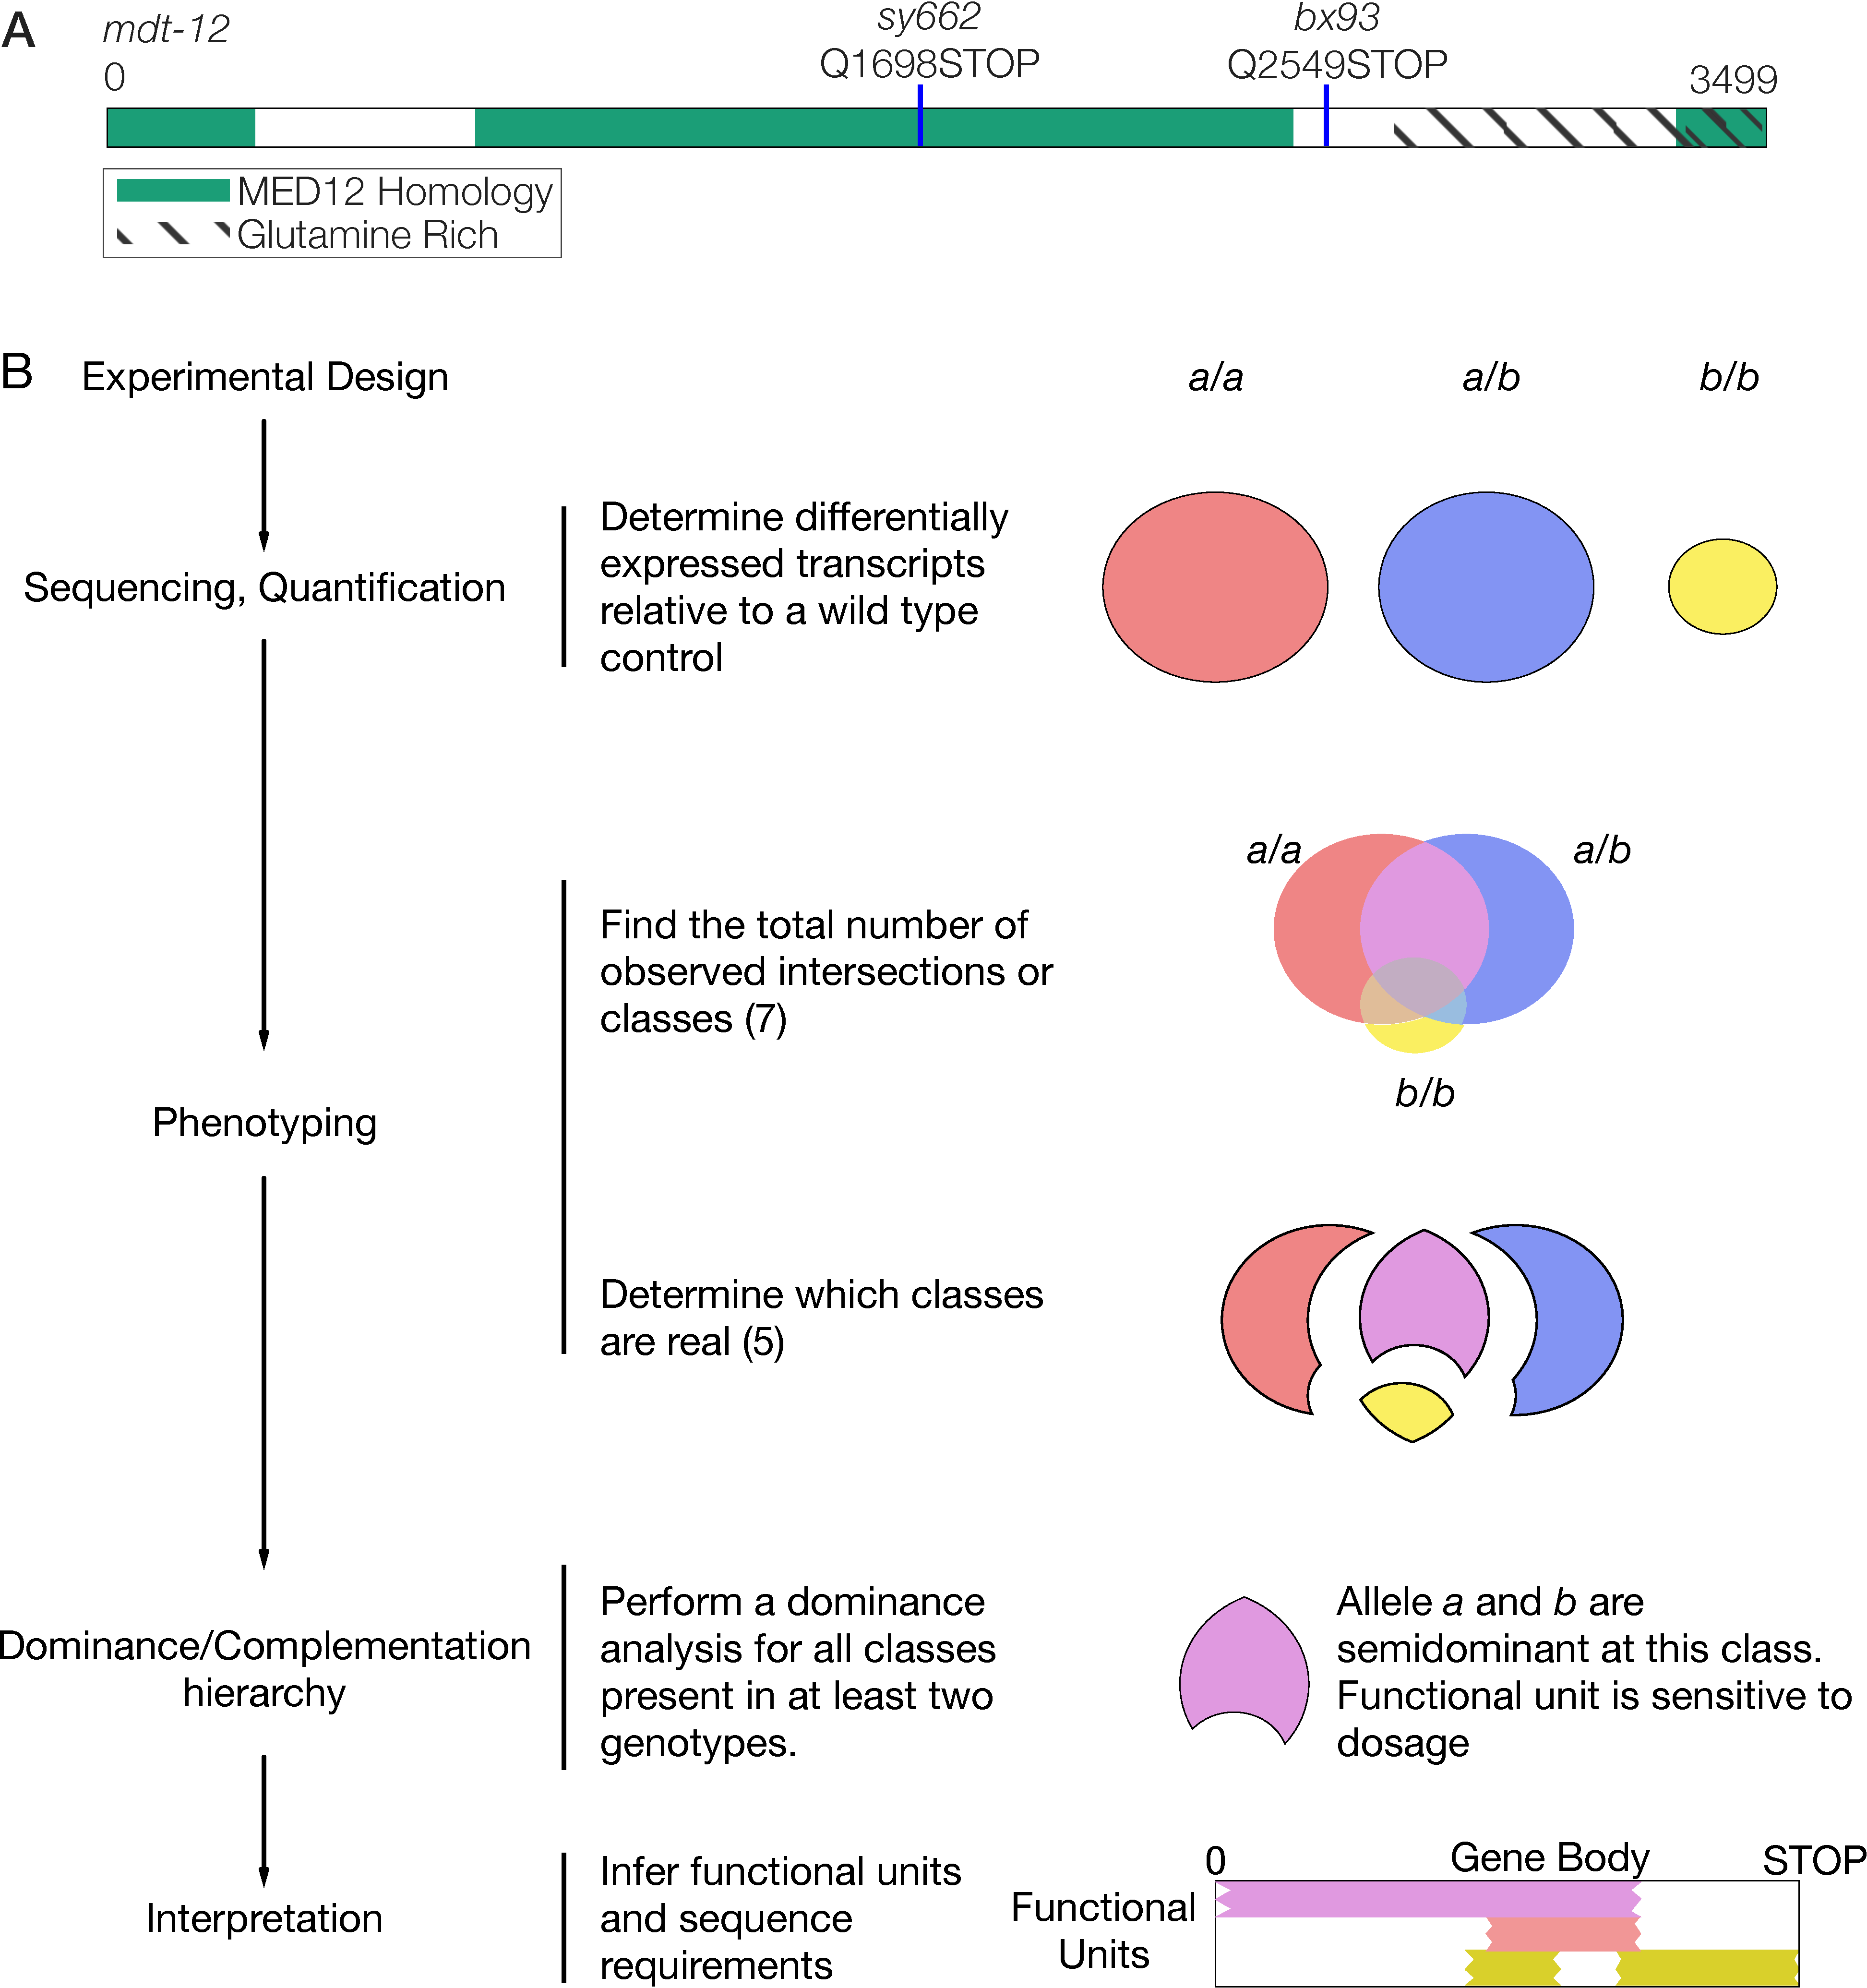
\includegraphics[width=\textwidth]{../../figs/Flowchart_Conceptual.pdf}
  \caption{
  \textbf{A} Protein sequence of \dpy{}. The positions of the nonsense
  mutations used are shown.
  \textbf{B} Flowchart for an analysis of arbitrary allelic series. A set of
  alleles is selected, and the corresponding genotypes are sequenced.
  Independent phenotypic classes are then identified. For each phenotypic class,
  the alleles are ordered in a dominance/complementation hierarchy, which can
  then be used to infer functional units within the genes in question.}
\label{fig:flowchart}
\end{figure*}

By these criteria, we found \weakn{} genes differentially expressed in
\bx{} homozygotes, and \strongn{} differentially expressed genes in
\sy{} homozygotes (see
\href{https://wormlabcaltech.github.io/med-cafe/notebook/basic.html}{Basic
Statistics Notebook}). We also sequenced \emph{trans}-heterozygotes with the
genotype \gene{dpy-6(e14) mdt-12(bx93)/+ mdt-12(sy622)}, and found \transn{}
differentially expressed genes.

We used a false hit analysis to identify four non-overlapping phenotypic
classes. We use the term genotype-specific to refer to groups of
transcripts that perturbed in one mutant. We use the term
genotype-associated to refer to those groups of transcripts  perturbed in two or
more mutants. The \textbf{\sy{}-associated} phenotypic class consisted
of 720 genes differentially expressed in \sy{} homozygotes and in
\emph{trans}-heterozygotes, but which had wild-type expression in \bx{}
homozygotes. The \textbf{\bx{}-associated} phenotypic class contains 403
genes differentially expressed in all genotypes. We also identified a
\textbf{\sy{}-specific} phenotypic class (1,841 genes) and a
\textbf{\emph{trans}-heterozygote-specific} phenotypic class (1,226 genes; see
the
\href{https://wormlabcaltech.github.io/med-cafe/notebook/phenotypic_classes.html}{
Phenotypic Classes Notebook}).
\todo[inline]{Note: the bx93-associated class is actually 3 classes merged
together. 2 of these classes aren't DE in all 3 genotypes (only 2 each), but my
analyses strongly suggest this is the result of false negatives}

We measured allelic dominance for each class. The \sy{} allele is
completely recessive to the \bx{} for the \sy{}-specific phenotypic
class. The \sy{} and \bx{} alleles are semidominant ($d_{bx93} =
0.51$) to each other for the \sy{}-associated phenotypic class. The
\bx{} allele is largely  dominant over the \sy{} allele
($d_{bx93}=0.81$; see Table~\ref{tab:dom}).

\begin{table}
  \centering
  \begin{tabular}{lc}
    \toprule
    Phenotypic Class & Dominance\\
    \midrule
    \sy{}-specific & $1.00\pm0.00$\\
    \sy{}-associated & $0.51\pm0.01$\\
    \bx{}-associated & $0.81\pm0.01$\\
    \bottomrule
    % \midrule{}
  \end{tabular}
  \caption{Dominance analysis for the \dpy{/MDT12} allelic series. Dominance
  values closer to 1 indicate \bx{} is dominant over \sy{}, whereas 0 indicates
  \sy{} is dominant over \bx{}.}
\label{tab:dom}

\end{table}

% \section*{Discussion}
% \label{sec:conclusions}
Our results suggest the existence of various functional units in \dpy{/MDT12}
(see Fig.~\ref{fig:domains}). The \sy{}-specific phenotypic class is likely
controlled by a single functional unit, functional unit 1 (FC1), and the
\sy{}-associated phenotypic class is likely controlled by a second
functional unit, functional unit 2 (FC2). It is unlikely that these units are
identical because their dominance behaviors are very different. The \bx{}
allele was largely dominant over the \sy{} allele for the
\bx{}-associated class, but gene expression in this class was perturbed in
both homozygotes. The perturbations were greater for \sy{} homozygotes
than for \bx{} homozygotes. This behavior can be explained if the
\bx{}-associated class is controlled jointly by two distinct effectors,
functional units 3 and 4 (FC3, FC4, see Fig.~\ref{fig:domains}). A rigorous
examination of this model will require studying alleles that mutate the region
between Q1689 and Q2549 using homozygotes and \emph{trans}-heterozygotes.

% Future work should be able to
% establish how many functional units exist in total, and how they may interact
% to drive gene expression.

\begin{figure}
  \centering{}
  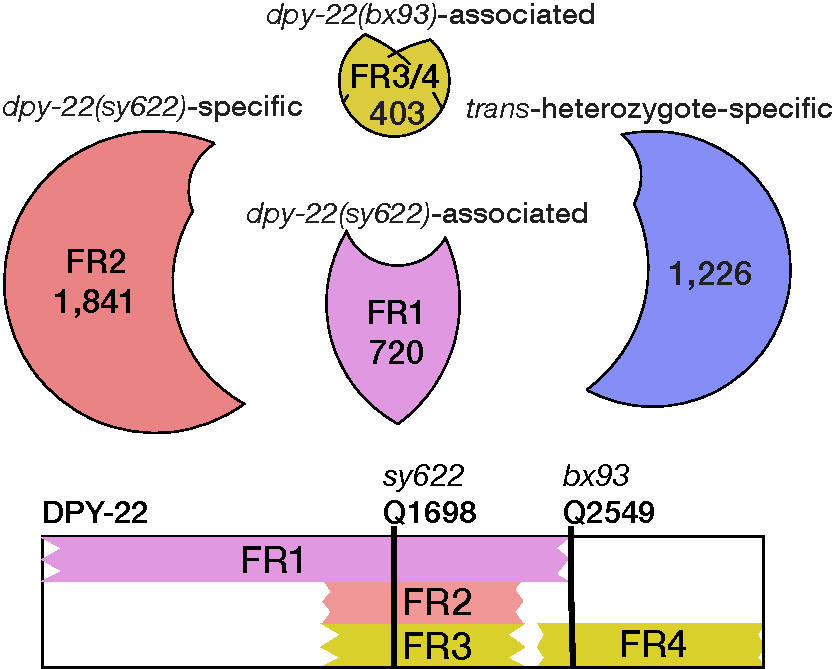
\includegraphics[width=0.5\textwidth]{../../figs/inferred_domains.pdf}
  \caption{
    The functional units associated with each phenotypic class can be
    mapped to intragenic locations. The beginning and end positions of
    these functional units are unknown,
    so edges are drawn as ragged lines. Thick horizontal lines show the
    limit where each function could end, if known. We postulate that the
    \bx{}-associated class is controlled by two functional units, FC3 and
    FC4, in the tail region of this gene. FC2 and FC3 may be redundant.
  }
\label{fig:domains}
\end{figure}

We also found a class of transcripts that had perturbed levels in
\emph{trans}-heterozygotes only; its biologicla significance is unclear.
Phenotypes unique to \emph{trans}-heterozygotes are often the result of physical
interactions such as homodimerization, or dosage reduction of a toxic
product~\cite{Yook2005}. In the case of \dpy{/MDT12} orthologs, how either mechanism
could operate is not obvious, since the \protein{mdt-12} is expected to assemble
in a monomeric manner into the CKM.\@ Massive single-cell sequencing of \cel{}
has recently been reported~\cite{Cao2017}. When this technique becomes
cost-efficient, single-cell profiling of these genotypes may provide information
that complements the whole-organism expression phenotypes, perhaps explaining
the origin of this phenotype.

Transcriptomic phenotypes generate large amounts of differential gene expression
data, so false positive and false negative rates can lead to spurious phenotypic
classes whose putative biological significance is badly misleading. Such
artifacts are particularly likely for small phenotypic classes, which should be
viewed with skepticism. Notably, errors of interpretation cannot be avoided by
setting a more stringent $q$-value cut-off; doing so will decrease the
false positive rate, but increase the false negative rate, which will in turn
produce smaller phenotypic classes than expected. Our method avoids this pitfall
by using total error rate estimates to assess the plausibility
of each class. These conclusions are of broad significance to research where
highly multiplexed measurements are compared to identify similarities and
differences in the genome-wide behavior of a single variable under multiple
conditions.

We have shown that transcriptomes can be used to study allelic series in the
context of a large, pleiotropic gene. We identified separable phenotypic classes
that would otherwise be obscured by other methods, correlated
each class to a functional unit, and identified sequence requirements for each
unit. Given the importance of allelic series for characterizing genetic
pathways, we are optimistic that this method will be a useful addition to the
geneticists arsenal.


\section*{Methods}
\label{sec:methods}
Methods, including statements of data availability and any associated
accession codes and references, are available in the online version of
the paper.

\subsection*{Strains used}
Strains used were N2 wild-type (Bristol),
PS4087 \gene{mdt-12(sy622)},
PS4187 \gene{mdt-12(bx93)},
%line break inserted below because \gene{...} doesn't linebreak well
and PS4176\\ \gene{dpy-6(e14) mdt-12(bx93)/ + mdt-12(sy622)}.
Lines were grown on standard nematode growth media (NGM) Petri plates seeded
with OP50 \ecol{} at 20\degree{}C~\cite{Brenner1974}.

\subsection*{Strain synchronization, harvesting and RNA sequencing}
Strains were synchronized by bleaching P$_0$'s into virgin S. basal (no
cholesterol or ethanol added) for 8--12 hours. Arrested L1 larvae were placed in
NGM plates seeded with OP50 at 20\degree{}C and grown to the young adult stage
(assessed by vulval morphology and lack of embryos). RNA extraction was
performed as described in~\cite{AngelesAlboresHIF} and sequenced using a
previously described protocol~\cite{Angeles-Albores2017}.

\subsection*{Read pseudo-alignment and differential expression}
Reads were pseudo-aligned to the \cel{} genome (WBcel235) using
Kallisto~\cite{Bray2016}, using 200 bootstraps and with the sequence bias
(\texttt{--seqBias}) flag. The fragment size for all libraries was set to 200
and the standard deviation to 40. Quality control was performed on a subset of
the reads using FastQC, RNAseQC, BowTie and
MultiQC~\cite{Andrews2010,Deluca2012,Langmead2009,Ewels2016}. All libraries had
good quality scores.

Differential expression analysis was performed using
Sleuth~\cite{Pimentel2016a}. We used a general linear model to identify
genes that were differentially expressed between wild-type and mutant libraries.
To increase our statistical power, we pooled young adult wild-type replicates
from other published~\cite{AngelesAlboresHIF,Angeles-Albores2017} and unpublished
analysis adjusting for batch effects.
% All wild-type replicates were collected at the same stage (young
% adult). In total, we had 10 wild-type replicates from 4 different batches, which
% heightened our statistical power. Batch effects were smaller than
% between-genotype effects, as assessed by principal component analysis (PCA),
% except when switching between samples constructed by different library methods.
% Wild-type samples constructed using the same library method clustered together
% and away from all other mutant samples. However, clustering wild-type samples by
% themselves revealed that the samples clusters correlated with the person who
% collected them. Therefore, we added batch correction terms to our model to
% account for batch effects from library construction as well as from the person
% who collected the samples.

% \subsection*{Non-parametric bootstrap}
% We performed non-parametric bootstrap testing to identify whether two
% distributions had the same test statistic using $10^6$ bootstraps.
% % Briefly, the two datasets were mixed,
% % and samples were selected at random with replacement from the mixed population
% % into two new datasets. We calculated the difference in the means of these new
% % datasets. We iterated this process $10^6$ times. To calculate a $p$-value that
% % the null hypothesis is true, we identified the number of times a difference in
% % the means of the simulated populations was greater than or equal to the observed
% % difference in the means of the real population. We divided this result by $10^6$
% % to complete the calculation for a $p$-value.
% If no statistics equal to or greater than the observed statistic was observed,
% we reported the $p$-value as $p<10^{-6}$. Otherwise, we reported
% the exact $p$-value. We chose to reject the null hypothesis that the means of
% the two datasets are equal to each other if $p < 0.05$.

\subsection*{False hit analysis}
To accurately count phenotypes, we developed a false hit algorithm (see
Algorithm~\ref{alg:false}). We implemented this algorithm for three-way
comparisons. We set our signal-to-noise threshold, $\alpha$, to 4 after random
benchmarking showed that this threshold performs well when false positive
and negative rates are close to 10\%. Using this threshold, the algorithm can
correctly identify genotype-specific classes with 75\% accuracy if the classes
contain $>800$ transcripts. Our method can identify when genotype-specific
classes are empty with extremely high precision. Determining whether a
genotype-specific class is real is most difficult when the class contains
50--500 transcripts. False negative rates for genotype-associated classes are
extremely low using this method for classes with any number of transcripts.
However, false positive rates are on the order of 30\%. 


\begin{algorithm}[H]
\label{alg:false}
  \DontPrintSemicolon{}

  \KwData{$\mathbf{M}_{obs} =  \{N_l\}$, an observed set of classes, where each
  class is labelled by $l\in L$ and is of size $N_l$. $f_p, f_n$, the false
  positive and negative rates respectively. $\alpha$, the signal-to-noise
  threshold for acceptance of a class.}
  \KwResult{$\mathbf{M}_{reduced}$, a reduced model that fits the data.}
  \BlankLine{}
  \Begin{
    \emph{Define a minimal set to initialize the reduced model}\;
    $\mathbf{K} = \{\min_{l \in L} N_l\}$\;

    \emph{Refine the model until the model converges or iterations max out}\;
    $i \leftarrow 0$\;
    $\mathbf{K_{prev}} \leftarrow \emptyset$\;
    \While{$(i < i_{\max})~|~(\mathbf{K_{prev}} \neq \mathbf{K}$)}{
      $\mathbf{K_{prev}} \leftarrow \mathbf{K}$\;

      \emph{Define a noise function to estimate error flows in
            $\mathbf{K}$}\;
      $\mathbf{F} \leftarrow \textrm{noise}(\mathbf{K}, f_p, f_n)$\;

      \For{$l \in L$}{
          \emph{Calculate signal to noise for each labelled class}\;
          \emph{False negatives can result in $\lambda < 0$}\;
          $\lambda_l \leftarrow \mathbf{M}_{obs, l}/F_{l}$\;
          % \emph{Use classes with high $\lambda_l$ to refine the model}\;
              \If{$(\lambda > \alpha)~|~(\lambda < 0)$}{
                $\mathbf{K}_l \leftarrow \mathbf{M}_{obs, l}$\;
              } %if
          } % end for
        $i++$
    } % end while
  } % end begin

  \emph{Return the reduced model}\;
  \Return{$\mathbf{K}$}

  \caption{False Hit Algorithm}
\end{algorithm}

\subsection*{Dominance analysis}
\label{subsec:dominance}
We modeled allelic dominance as a weighted average of allelic activity:
% our model proposed that $\beta$ coefficients of the heterozygote,
% $\beta_{a/b,i,\text{Pred}}$, could be modeled as a linear combination of the
% coefficients of each homozygote:
\begin{equation}
  \beta_{a/b,i,\text{Pred}}(d_a) = d_a\cdot \beta_{a/a,i} +
                                   (1-d_a)\cdot \beta_{b/b,i},
\end{equation}
where $\beta_{k/k, i}$ refers to the $\beta$ value of the $i$th isoform in a
genotype $k/k$, and $d_a$ is the dominance coefficient for allele $a$.

To find the parameters $d_a$ that maximized the probability of observing the
data, we found the parameter, $d_a$, that maximized the equation:
\begin{equation}
    P(d_a|D,H,I) \propto \prod_{i \in S}
                   \exp{-\frac{{(\beta_{a/b,i,\text{Obs}} -
                                \beta_{a/b,i,\text{Pred}}(d_a))}^2}{
                                2\sigma_i^2}}
\end{equation}
where $\beta_{a/b,i,\text{Obs}}$ was the coefficient associated with the $i$th
isoform in the \emph{trans}-het $a/b$ and $\sigma_i$ was the standard error of
the $i$th isoform in the \emph{trans}-heterozygote samples as output by
Kallisto. $S$ is the set of isoforms that participate in the regression (see
main text). This equation describes a linear regression which was solved
numerically.

\subsection*{Code}
Code was written in Jupyter notebooks~\cite{Perez2007} using the Python
programming language. The Numpy, pandas and scipy libraries were used for
computation~\cite{VanDerWalt2011,McKinney2011,Oliphant2007} and the matplotlib
and seaborn libraries were used for data visualization~\cite{Hunter2007,Waskom}.
Enrichment analyses were performed using the WormBase Enrichment
Suite~\cite{Angeles-Albores2016}. For all enrichment analyses, a $q$-value of
less than $10^{-3}$ was considered statistically significant. For gene ontology
enrichment analysis, terms were considered statistically significant only if
they also showed an enrichment fold-change greater than 2.

\subsection*{Data Availability}
Raw and processed reads were deposited in the Gene Expression Omnibus. Scripts
for the entire analysis can be found with version control in our Github
repository, \url{https://github.com/WormLabCaltech/med-cafe}. A user-friendly,
commented website containing the complete analyses can be found at
\url{https://wormlabcaltech.github.io/med-cafe/}. Raw reads and quantified
abundances for each sample were deposited at the NCBI Gene Expression Omnibus
(GEO)~\cite{Edgar2002} under the accession code GSE107523
(\url{https://www.ncbi.nlm.nih.gov/geo/query/acc.cgi?acc=GSE107523}).

\section*{Acknowledgements}
This work was supported by HHMI with whom PWS was an investigator, by the
Millard and Muriel Jacobs Genetics and Genomics Laboratory at California
Institute of Technology, and by the NIH grant U41 HG002223. This article
would not be possible without help from Dr.\ Igor Antoshechkin and Dr.\ Vijaya
Kumar who performed the library preparation and sequencing.
% We would like to
% thank Carmie Puckett Robinson for the unpublished Dpy transcriptional
% signature.
Han Wang, Hillel Schwartz, Erich Schwarz, Porfirio Quintero and
Carmie Puckett Robinson provided valuable input throughout the project.

%This is where your bibliography is generated.
\bibliography{citations}
\bibliographystyle{naturemag}

\end{document}
